\subsection{The {\tt NCR:} module}\label{sect:NCRData}

This component of DONJON is dedicated to the interpolation of {\sc microlib} and
{\sc macrolib} data from a {\sc multicompo} object, the reactor database produced by {\tt COMPO:}.
A set of {\sl global} and/or {\sl local parameters} are defined for each material mixture and
used as multi-dimensional interpolation variables.

\vskip 0.02cm

The calling specifications are:

\begin{DataStructure}{Structure \dstr{NCR:}}
\dusa{MLIB}~\moc{:=}~\moc{NCR:}~$[~\{$~\dusa{MLIB} $|$ \dusa{MLIB2}~$\}~]$ \dusa{CPONAM1} $[[$~\dusa{CPONAM2}~$]]~[$~\dusa{MAPFL}~$]$~\moc{::}~\dstr{ncr\_data} \\
\end{DataStructure}

\noindent where
\begin{ListeDeDescription}{mmmmmmm}

\item[\dusa{MLIB}] {\tt character*12} name of a {\sc microlib} (type {\tt L\_LIBRARY}) or {\sc macrolib} (type {\tt L\_MACROLIB}) containing the interpolated
data. If this object also appears on the RHS of structure \dstr{NCR:}, it is open in modification mode and updated.

\item[\dusa{MLIB2}] {\tt character*12} name of an optional {\sc microlib} object whose content is copied on \dusa{MLIB}.

\item[\dusa{CPONAM1}] {\tt character*12} name of the {\sc lcm} object containing the
{\sc multicompo} data structure ({\tt L\_MULTICOMPO} signature).

\item[\dusa{CPONAM2}] {\tt character*12} name of an additional {\sc lcm} object containing an auxiliary
{\sc multicompo} data structure ({\tt L\_MULTICOMPO} signature). This object is optional.

\item[\dusa{MAPFL}] {\tt character*12} name of the {\sc map} object containing fuel regions description, global and local parameter
information (burnup, fuel/coolant temperatures, coolant density, etc). Keyword \moc{TABLE} is expected in \dstr{ncr\_data}.

\item[\dusa{ncr\_data}] input data structure containing interpolation information (see \Sect{descncr}).

\end{ListeDeDescription}

\subsubsection{Interpolation data input for module {\tt NCR:}}\label{sect:descncr}

\vskip -0.5cm

\begin{DataStructure}{Structure \dstr{ncr\_data}}
$[$~\moc{EDIT} \dusa{iprint}~$]$ \\
$[$~\moc{ALLX} \dusa{nbfuel}~$]~[$~\moc{RES} $]~[$~\moc{PURE} $]$ \\
$[~\{$~\moc{MACRO}~$|$~\moc{MICRO}~$\}~]~[~\{$~\moc{LINEAR}~$|$~\moc{CUBIC}~$\}~]~[$~\moc{LEAK}~\dusa{b2}~$]$ \\
$[$~\moc{NMIX} \dusa{nmixt}~$]$ \\
$\{~[[$~\moc{COMPO} \dusa{CPONAM} \dusa{NAMDIR} \dstr{descintf}~$]]$ \\ 
$~|~[[$~\moc{TABLE} \dusa{CPONAM} \dusa{NAMDIR} $[$ \dusa{namburn} $]$ \dstr{descintf} ~$]]~\}$ \\
{\tt ;}
\end{DataStructure}

\noindent where
\begin{ListeDeDescription}{mmmmmmmm}

\item[\moc{EDIT}] keyword used to set \dusa{iprint}.

\item[\dusa{iprint}] index used to control the printing in module {\tt NCR:}. =0 for no print; =1 for minimum printing (default value).

\item[\moc{ALLX}] keyword used to register the region number of each isotope before merging. This option is useful if the same keyword has been specified in \moc{EDI:} and \moc{COMPO:} before.

\item[\dusa{nbfuel}] number of fuel rings used for micro-depletion calculations.

\item[\moc{RES}] keyword indicating that the interpolation is done only for the microscopic cross sections and not for the isotopic densities. In this case, a RHS {\sc microlib} must be defined and the number densities are recovered from it. This option is useful for micro-depletion applications. {\bf Important note:} It is possible to force interpolation of some isotopic densities with \moc{RES} option if these
isotopes are explicitely specified with a ``\moc{*}'' flag after \moc{MICRO} keyword in \dusa{descintf} input data structure (see \Sect{descintf}).

\item[\moc{PURE}] keyword indicating that the interpolation is a pure linear combination of terp factors. The fission spectra are {\sl not}
renormalized. By default, non-linear effects are produced by renormalization operations.

\item[\moc{MACRO}] keyword indicating that \dusa{MLIB} is a {\sc macrolib}.

\item[\moc{MICRO}] keyword indicating that \dusa{MLIB} is a {\sc microlib} (default option). Object \dusa{MLIB} contains an embedded {\sc macrolib}, but the CPU time required to obtain it is longer.

\item[\moc{LINEAR}] keyword indicating that interpolation of the {\sc multicompo} uses linear Lagrange polynomials (default option).

\item[\moc{CUBIC}] keyword indicating that interpolation of the {\sc multicompo} uses the Ceschino method
with cubic Hermite polynomials, as presented in Ref.~\citen{Intech2011}.

\item[\moc{LEAK}] keyword used to introduce leakage in the embedded {\sc macrolib}. This option should only be used for non-regression tests.

\item[\dusa{b2}] the imposed buckling corresponding to the leakage.

\item[\moc{NMIX}] keyword used to define the maximum number of material mixtures. This information is required  only if \dusa{MLIB} is created.

\item[\dusa{nmixt}] the maximum number of mixtures (a mixture is characterized by a distinct set of 
macroscopic cross sections) the {\sc macrolib} may contain. The default value is \dusa{nmixt} $=0$ or the value recovered from \dusa{MLIB} if it appears on
the RHS of structure \dstr{NCR:}.

\item[\moc{COMPO}] keyword used to set \dusa{CPONAM} and to define each global and local parameter.

\item[\moc{TABLE}] keyword used to set \dusa{CPONAM} and to recover some global and local parameter from a {\sc map} object named \dusa{MAPFL}.

\item[\dusa{CPONAM}] {\tt character*12} name of the {\sc lcm} object containing the
{\sc multicompo} data structure where the interpolation is performed. This name must be set in the RHS of structure \dstr{NCR:}.

\item[\dusa{NAMDIR}] access the {\sc multicompo} structure of \dusa{CPONAM} from the sub-directory named \dusa{NAMDIR}.
This value must be set equal to {\tt 'default'} if not previously defined by a {\tt STEP UP} keyword in module {\tt COMPO}.

\item[\dusa{namburn}] name of the parameter for burnup (or irradiation) in the sub-directory named \dusa{NAMDIR}.
This value is defined if option \moc{TABLE} is set {\sl and} if burnup (or irradiation) is to be considered as parameter.

\item[\dusa{descintf}] input data structure containing interpolation information relative to the {\sc multicompo} data structure named \dusa{CPONAM} (see \Sect{descintf}).

\end{ListeDeDescription}

\subsubsection{Defining local and global parameters}\label{sect:descintf}

\vskip -0.5cm

If a {\sc map} object is defined on the RHS of structure \dstr{NCR:}, and if the \moc{TABLE} keyword is set, some information required to set the interpolation points is found in this object. In this case, the {\tt NCR:} operator search the {\sc multicompo} object for global or local parameters  having an arbitrary name specified in the {\sc map} object or set directly in  this module. Note that any parameter's value set directly in this module prevails on a value stored in the \dusa{MAPFL} object.

Each instance of \dusa{descintf} is a data structure specified as

\begin{DataStructure}{Structure \dstr{descintf}}
$[[$~\moc{MIX} \dusa{imix}~$[~\{$~\moc{FROM}~\dusa{imixold}~$|$~\moc{USE}~$\}~]$ \\
~~~~~~$[~\{$~\moc{TIMAV-BURN} $|$ \moc{INST-BURN} $|$ \moc{AVG-EX-BURN}~\dusa{ivarty}~$\}~]$ \\
~~~~~~$[[~\{$~\moc{SET} $|$ \moc{DELTA} $|$ \moc{ADD}~$\}~\}~[~\{$ \moc{LINEAR} $|$ \moc{CUBIC}~$\}~]$ \dusa{PARKEY} $\{$~\dusa{val1} $|$ \moc{MAP}~$\}~[~\{$~\dusa{val2} $|$ \moc{MAP}~$\}~]$ \\
~~~~~~~~~~~~$[$~\moc{REF} $[[$~\dusa{PARKEY}~$\{$~\dusa{valref} $|$ \moc{SAMEASREF}~$\}$~$]]$~\moc{ENDREF}~$]~]]$  \\
~~~~~~$[$~\moc{MICRO}~$\{$~\moc{ALL} $|$ \moc{ONLY}~$\}~[[$~\dusa{HISO} $\{$ \dusa{conc} $|$ \moc{*} $\}~]]~]$ \\
\moc{ENDMIX}~$]]$
\end{DataStructure}

\noindent where
\begin{ListeDeDescription}{mmmmmmmm}

\item[\moc{MIX}] keyword used to set \dusa{imix}. Discontinuity factor information present in the Multicompo is interpolated as mixture~1 values.

\item[\dusa{imix}] index of the mixture that is to be created in the {\sc microlib} and {\sc macrolib}.

\item[\moc{FROM}] keyword used to set the index of the mixture in the {\sc multicompo} object.

\item[\dusa{imixold}] index of the mixture that is recovered in the {\sc multicompo} object. By default, \dusa{imixold}$=1$.

\item[\moc{USE}] keyword used to set the index of the mixture in the {\sc multicompo} object equal to \dusa{imix}.

\item[\moc{TIMAV-BURN}] keyword used to compute time-averaged cross-section information. This option is available {\sl only if} a \dusa{MAPFL} object is set.
By default, the type of calculation (\moc{TIMAV-BURN} or \moc{INST-BURN}) is recovered from the \dusa{MAPFL} object.

\item[\moc{INST-BURN}] keyword used to compute cross-section information at specific bundle burnups. This option is available {\sl only if} a \dusa{MAPFL} object is set.
By default, the type of calculation (\moc{TIMAV-BURN} or \moc{INST-BURN}) is recovered from the \dusa{MAPFL} object.

\item[\moc{AVG-EX-BURN}] keyword used to compute the derivatives of cross-section information relative to the exit burnup of a single combustion zone. The derivatives are computed using Eq.~(3.3) of Ref.~\citen{chambon}, written as
$$
{\partial \bar\Sigma_x\over \partial B_j^{\rm e}}={1\over B_j^{\rm e}\, (B_{j,k}^{\rm eoc}-B_{j,k}^{\rm boc})}
\left[- \int_{B_{j,k}^{\rm boc}}^{B_{j,k}^{\rm eoc}}dB \, \Sigma_x(B)+B_{j,k}^{\rm eoc}\, \Sigma_x(B_{j,k}^{\rm eoc})-B_{j,k}^{\rm boc}\, \Sigma_x(B_{j,k}^{\rm boc})\right]
$$

\noindent where $B_{j,k}^{\rm boc}$, $B_{j,k}^{\rm eoc}$, and $B_j^{\rm e}$ are the beginning of cycle burnup of bundle $\{j,k\}$, end of cycle burnup of bundle $\{j,k\}$ and exit burnup of channel $j$. This option is available {\sl only if} a \dusa{MAPFL} object is set.
By default, the type of calculation (\moc{TIMAV-BURN} or \moc{INST-BURN}) is recovered from the \dusa{MAPFL} object.

\item[\dusa{ivarty}] index of the combustion zone for differentiation of cross-section information.

\item[\moc{SET}] keyword used to indicate a simple interpolation at \dusa{val1} or an averaging between \dusa{val1} and \dusa{val2}. The result $\sigma_{\rm ref}$ is also used as the reference value when the \moc{ADD} is used. Note: see at the ending note of this section for a detailed description and examples.

\item[\moc{DELTA}] keyword used to indicate a delta-sigma calculation between \dusa{val2} and \dusa{val1}
(i.e., $\Delta\sigma_{\rm ref}=\sigma_{\rm val2}-\sigma_{\rm val1}$ is computed). This keyword can be used only once in each mixture data block (initiated
with a \moc{MIX} keyword).  Note: see at the ending note of this section for a detailed description and examples.

\item[\moc{ADD}] keyword used to indicate a delta-sigma calculation between \dusa{val2} and \dusa{val1} is added to the reference value
(i.e., $\Delta\sigma=\sigma_{\rm val2}-\sigma_{\rm val1}$ is used as contribution, $\sigma_{\rm ref}+\Delta\sigma$ or $\Delta\sigma_{\rm ref}+\Delta\sigma$ is returned). Note: see at the ending note of this section for a detailed description and examples.

\item[\moc{LINEAR}] keyword indicating that interpolation of the {\sc multicompo} for parameter \dusa{PARKEY} uses linear Lagrange
polynomials. It is possible to set different interpolation modes to different parameters. By default, the interpolation mode is set in Sect.~\ref{sect:descncr}.

\item[\moc{CUBIC}] keyword indicating that interpolation of the {\sc multicompo} for parameter \dusa{PARKEY} uses the Ceschino method
with cubic Hermite polynomials, as presented in Ref.~\citen{Intech2011}. By default, the interpolation mode is set in Sect.~\ref{sect:descncr}.

\item[\dusa{PARKEY}] {\tt character*12} user-defined keyword associated to a global
or local parameter to be set.

\item[\dusa{val1}] value of a global or local parameter used to interpolate.  \dusa{val1} is the initial value of this parameter in case an average is required. \dusa{val1} can be an integer, real or string value.

\item[\dusa{val2}] value of the final global or local parameter. By default, a simple interpolation is performed, so that \dusa{val2}$=$\dusa{val1}. \dusa{val2} is always a real value with \dusa{val2}$\ge$\dusa{val1}.

\item[\moc{MAP}] keyword used to indicate that the value of parameter \dusa{val1} or the second value for the $\Delta\sigma$ calculation is
recovered from \dusa{MAPFL}, i.e. the {\sc map} object containing fuel regions description.

\item[\moc{REF}] keyword only available together with the \moc{ADD} option. It is used to set all the other variable values when a $\Delta$ contribution is performed for one variable.  

\item[\dusa{valref}] value of the reference parameter, when it is directly given by the user. Note that there is no default value.

\item[\moc{SAMEASREF}] keyword used to specify that the reference value will be the same as in the refence case, i.e. for the $\sigma_{\rm ref}$ computation.

\item[\moc{ENDREF}] keyword only available together with the \moc{ADD} option. It is used to specify that all the other variable values which are required are given.  

\item[\moc{MICRO}] keyword used to set the number densities of some isotopes present in the {\sc multicompo} object. The data statement ``\moc{MICRO} \moc{ALL}" is used by default.

\item[\moc{ALL}] keyword to indicate that all the isotopes present in the  {\sc multicompo} object will be used in the {\sc microlib} and {\sc macrolib} objects. Concentrations of these isotopes will be recovered from the {\sc multicompo} object
or set using the ``\dusa{HISO} \dusa{conc}" data statement.

\item[\moc{ONLY}] keyword to indicate that only the isotopes set using the ``\dusa{HISO} \dusa{conc}" data statement will be used in the {\sc microlib} and {\sc macrolib} objects.

\item[\dusa{HISO}] {\tt character*8} name of an isotope.

\item[\dusa{conc}] user-defined value of the number density (in $10^{24}$ particles per ${\rm cm}^3$) of the isotope.

\item[\moc{*}] the value of the number density for isotope \dusa{HISO} is recovered from the {\sc multicompo} object.

\item[\moc{ENDMIX}] end of specification keyword for the material mixture.

\end{ListeDeDescription}


\subsubsection{Interpolation in the parameter grid}


The following example corresponds to a delta-sigma computation in mixture 1 corresponding to a perturbation. Note that in this case, the \moc{MACROLIB} object  may content negative cross-section. 
\begin{verbatim}
MACROLIB := NCR: CPO ::
   EDIT 40 NMIX 1 MACRO COMPO CPO default
   MIX 1  !(* delta sigma contribution *)
          SET 'CELL' '3D'
          DELTA 'PITCH' 0.0 1.0
   ENDMIX
;
\end{verbatim}

When the number of parameters used for the interpolation is increased, all the lattice computations corresponding to all the combinations of parameters may not be done for computation time reasons. In this case, some approximations may be required. The choice for the \moc{SET}, \moc{DELTA} and \moc{ADD} is then dependent of the structure of the database (i.e. how the database grid of possibilities is filled). When a {\sc map} object containing fuel regions description is used, the problem become even more complex, because values have to be automatically changed for all bundles. In order to clarify all the different possibilities and limitations dependently of the database structure, we will use a 3 parameter case. The paramaters are referenced by 'A', 'B' and 'C'. But before we explain the different cases, we want to remind that the interpolation factors are computed on each axis seperatly.

The first case corresponds to a complete grid, represented by a gray paralepiped on Fig. \ref{figNCRGRIDINS} and \ref{figNCRGRIDTA}. The
figure \ref{figNCRGRIDINS} shows that the interpolated value in point $V$ can be obtained directly without {\sc map} object. For time-average (TA) computation, lets assume that the parameter 'B' represents the burnup (and keep this convention for other database structure also). In this case the figure \ref{figNCRGRIDTA} shows also that the direct interpolation can be done to compute an average value between the points $V'$ and $V$. Note that the TA burnups are stored in the {\sc map} object, and are then recovered automatically.

The second case corresponds to a partial grid where all the lattice computations have been perfomed for several pairs of parameters, which are represented as the gray rectangles on Fig. \ref{figNCRPLANEINS} and \ref{figNCRPLANETA}. If we use the notations of Fig. \ref{figNCRPLANEINS} and \ref{figNCRPLANETA}, the best estimate interpolated values, $f$, we can get are given by: \\
$f=f(V)~\approx~f(V_B)+(f(V_{BA})-f(V_B))+(f(V_{BC})-f(V_B))=f(V_{BC})+(f(V_{BA})-f(V_B))=f(V_{BA})+(f(V_{BC})-f(V_B))$ for instataneous\\
$f=f(V',V)~\approx~f(V'_B,V_B)+(f(V'_{BA},V_{BA})-f(V'_B,V_B))+(f(V'_{BC},V_{BC})-f(V'_B,V_B))=f(V'_{BC},V_{BC})+(f(V'_{BA},V_{BA})-f(V'_B,V_B))=f(V'_{BA},V_{BA})+(f(V'_{BC},V_{BC})-f(V'_B,V_B))$ for TA\\
~~~~where $f(.,.)$ represents the average value between two points.

The third case corresponds to a minimal grid, where the lattice computations have been perfomed only for one parameter variation at a time. In this case, the grid is represented by the thick gray lines on the axis on Fig. \ref{figNCRAXEINS} and \ref{figNCRAXETA}. If we use the notations of Fig. \ref{figNCRAXEINS} and \ref{figNCRAXETA}, the best estimate interpolated values, $f$, we can get are given by: \\
$f=f(V)~\approx~f(V_0)+(f(V_A)-f(V_0))+(f(V_B)-f(V_0))+(f(V_C)-f(V_0))=f(V_B)+(f(V_A)-f(V_0))+(f(V_C)-f(V_0))$ for instataneous\\
$f=f(V',V)~\approx~f(V'_B,V_B)+(f(V_A)-f(V_0))+(f(V_C)-f(V_0))$ for TA\\
Note that the reference point ($V_0$ in the example) does not have to be the same for all parameters. Database structures such as represented on Fig \ref{figNCRAXEINSbis} can also been used. In this case, we even have two choices for the $\Delta f$ computation on axis 'A'. 

The last case is in fact a mix of cases 2 and 3. The gray rectangle and the gray line on Fig. \ref{figNCRPLAXINS} and \ref{figNCRPLAXTA} reprensent where all the lattice computations have been performed. With the notations used on those figures, one can write that the best estimate interpolated values, $f$, we can get are given by: \\
$f=f(V)~\approx~f(V_B)+(f(V_{BC})-f(V_B))+(f(V_A)-f(V_0))=f(V_{BC})+(f(V_A)-f(V_0))$ for instataneous\\
$f=f(V',V)~\approx~f(V'_B,V_B)+(f(V'_{BC},V_{BC})-f(V'_B,V_B))+(f(V_A)-f(V_0))=f(V'_{BC},V_{BC})+(f(V_A)-f(V_0))$ for TA\\
Note once again that the reference point ($V_0$ in the example) does not have to be the same for all parameters. Database structures such as represented on Fig \ref{figNCRPLAXINSbis} can also been used.
\clearpage

The input files will actually reflect the previous equations. However, they are different if the parameters are stored in a {\sc map} object, \dusa{MAPFL}, or provided directly by the user. For the case of one point interpolation (i.e. instantaneous), the input files will be: \\

\begin{center}
\tablefirsthead{%
\hline
case & all parameters explicitly set & all parameters in {\sc map}\\
\hline}
\tablehead{%
%\hline
%\multicolumn{3}{|l|}{\small\sl continued from previous page}\\
\hline
case & all parameters explicitly set & all parameters in {\sc map}\\
\hline}
\tabletail{%
\hline
\multicolumn{3}{|r|}{\small\sl continued on next page}\\
\hline}
\tablelasttail{\hline}
\bottomcaption{NCR inputs for instantaneous cases}

\begin{supertabular}{|p{0.1\textwidth}|p{0.4\textwidth}|p{0.4\textwidth}|}
%\begin{tabular}{|p{0.1\textwidth}|p{0.4\textwidth}|p{0.4\textwidth}|}
%\hline
%case & all parameters explicitly set & all parameters in {\sc map}\\
\hline
GRID (Fig. \ref{figNCRGRIDINS}) 
& \begin{verbatim}
MACROLIB := NCR: CPO ::
   NMIX 1 MACRO 
   COMPO CPO default
   MIX 1 
      SET 'A' <<va>>
      SET 'B' <<vb>>
      SET 'C' <<vc>>
   ENDMIX
;
\end{verbatim} 
& \begin{verbatim}
MACROLIB := NCR: CPO FMAP ::
   NMIX 1 MACRO 
   TABLE CPO default 'B' 
   MIX 1 
   ENDMIX
;
\end{verbatim} \\
\hline
PLANE (Fig. \ref{figNCRPLANEINS}) & 
\begin{verbatim}
MACROLIB := NCR: CPO ::
   NMIX 1 MACRO 
   COMPO CPO default
   MIX 1 
      SET 'A' <<va>>
      SET 'B' <<vb>>
      SET 'C' <<vc0>>
      ADD 'C' <<vc0>> <<vc>>
         REF  'A' <<va0>> 
              'B' <<vb>> ENDREF
!or           'B' SAMEASREF ENDREF
   ENDMIX
;
\end{verbatim} &
\begin{verbatim}
MACROLIB := NCR: CPO FMAP ::
   NMIX 1 MACRO 
   TABLE CPO default 'B' 
   MIX 1 
      SET 'C' <<vc0>>
      ADD 'C' <<vc0>> MAP
         REF  'A' <<va0>> 
              'B' SAMEASREF ENDREF
!or   SET 'A' <<va0>>
!or   ADD 'A' <<va0>> MAP
!or      REF  'C' <<vc0>> 
!or           'B' SAMEASREF ENDREF
   ENDMIX
;
\end{verbatim} \\
\hline
%\end{tabular}
%
%\begin{tabular}{|p{0.1\textwidth}|p{0.4\textwidth}|p{0.4\textwidth}|}
%\hline
%case & all parameters explicitly set & all parameters in {\sc map}\\
%\hline
AXE (Fig. \ref{figNCRAXEINS}) & 
\begin{verbatim}
MACROLIB := NCR: CPO ::
   NMIX 1 MACRO 
   COMPO CPO default
   MIX 1 
      SET 'A' <<va0>>
      SET 'B' <<vb>>
      SET 'C' <<vc0>>
      ADD 'A' <<va0>> <<va>>
         REF  'C' <<vc0>> 
              'B' <<vb0>> ENDREF
      ADD 'C' <<vc0>> <<vc>>
         REF  'A' <<va0>> 
              'B' <<vb0>> ENDREF
   ENDMIX
;
\end{verbatim} &
\begin{verbatim}
MACROLIB := NCR: CPO FMAP ::
   NMIX 1 MACRO 
   TABLE CPO default 'B' 
   MIX 1 
      SET 'A' <<va0>>
      SET 'C' <<vc0>>
      ADD 'A' <<va0>> MAP
         REF  'C' <<vc0>> 
              'B' <<vb0>> ENDREF
      ADD 'C' <<vc0>> MAP
         REF  'A' <<va0>> 
              'B' <<vb0>> ENDREF
   ENDMIX
;
\end{verbatim} \\
\hline
PLANE + AXE (Fig. \ref{figNCRPLAXINS}) & 
\begin{verbatim}
MACROLIB := NCR: CPO ::
   NMIX 1 MACRO 
   COMPO CPO default
   MIX 1 
      SET 'A' <<va0>>
      SET 'B' <<vb>>
      SET 'C' <<vc>>
      ADD 'A' <<va0>> <<va>>
         REF  'C' <<vc0>> 
              'B' <<vb0>> ENDREF
   ENDMIX
;
\end{verbatim} &
\begin{verbatim}
MACROLIB := NCR: CPO FMAP ::
   NMIX 1 MACRO 
   TABLE CPO default 'B' 
   MIX 1 
      SET 'A' <<va0>>
      ADD 'A' <<va0>> MAP
         REF  'C' <<vc0>> 
              'B' <<vb0>> ENDREF
   ENDMIX
;
\end{verbatim} \\
\hline
%\end{tabular}
\end{supertabular}
\end{center}

For the TA, the burnup variable has no other choice than to be stored in the {\sc map} object, \dusa{MAPFL}. Then the input files will be: \\

\begin{center}
\tablefirsthead{%
\hline
case & only the burnup in {\sc map} & all parameters in {\sc map}\\
\hline}
\tablehead{%
%\hline
%\multicolumn{3}{|l|}{\small\sl continued from previous page}\\
\hline
case & only the burnup in {\sc map} & all param. in {\sc map}\\
\hline}
\tabletail{%
\hline
\multicolumn{3}{|r|}{\small\sl continued on next page}\\
\hline}
\tablelasttail{\hline}
\bottomcaption{NCR inputs for TA cases}

\begin{supertabular}{|p{0.1\textwidth}|p{0.4\textwidth}|p{0.4\textwidth}|}
%\begin{tabular}{p{0.1\textwidth}|p{0.4\textwidth}|p{0.4\textwidth}}
%\hline
%case & only the burnup in {\sc map} & all parameters in {\sc map}\\
\hline
GRID (Fig. \ref{figNCRGRIDTA}) & 
\begin{verbatim}
MACROLIB := NCR: CPO FMAP ::
   NMIX 1 MACRO 
   TABLE CPO default 'B' 
   MIX 1 
      SET 'A' <<va>>
      SET 'C' <<vc>>
   ENDMIX
;
\end{verbatim} &
\begin{verbatim}
MACROLIB := NCR: CPO FMAP ::
   NMIX 1 MACRO 
   TABLE CPO default 'B' 
   MIX 1 
   ENDMIX
;
\end{verbatim} \\
\hline
PLANE (Fig. \ref{figNCRPLANETA}) & 
\begin{verbatim}
MACROLIB := NCR: CPO FMAP ::
   NMIX 1 MACRO 
   TABLE CPO default 'B' 
   MIX 1 
      SET 'A' <<va>>
      SET 'C' <<vc0>>
      ADD 'C' <<vc0>> <<vc>>
         REF  'A' <<va0>> 
              'B' SAMEASREF ENDREF
   ENDMIX
;
\end{verbatim} &
\begin{verbatim}
MACROLIB := NCR: CPO FMAP ::
   NMIX 1 MACRO 
   TABLE CPO default 'B' 
   MIX 1 
      SET 'C' <<vc0>>
      ADD 'C' <<vc0>> MAP
         REF  'A' <<va0>> 
              'B' SAMEASREF ENDREF
!or   SET 'A' <<va0>>
!or   ADD 'A' <<va0>> MAP
!or      REF  'C' <<vc0>> 
!or           'B' SAMEASREF ENDREF
   ENDMIX
;
\end{verbatim} \\
\hline
AXE (Fig. \ref{figNCRAXETA}) & 
\begin{verbatim}
MACROLIB := NCR: CPO FMAP ::
   NMIX 1 MACRO 
   TABLE CPO default 'B' 
   MIX 1 
      SET 'A' <<va0>>
      SET 'C' <<vc0>>
      ADD 'A' <<va0>> <<va>>
         REF  'C' <<vc0>> 
              'B' <<vb0>> ENDREF
      ADD 'C' <<vc0>> <<vc>>
         REF  'A' <<va0>> 
              'B' <<vb0>> ENDREF
   ENDMIX
;
\end{verbatim} &
\begin{verbatim}
MACROLIB := NCR: CPO FMAP ::
   NMIX 1 MACRO 
   TABLE CPO default 'B' 
   MIX 1 
      SET 'A' <<va0>>
      SET 'C' <<vc0>>
      ADD 'A' <<va0>> MAP
         REF  'C' <<vc0>> 
              'B' <<vb0>> ENDREF
      ADD 'C' <<vc0>> MAP
         REF  'A' <<va0>> 
              'B' <<vb0>> ENDREF
   ENDMIX
;
\end{verbatim} \\
\hline
PLANE + AXE (Fig. \ref{figNCRPLAXTA}) & 
\begin{verbatim}
MACROLIB := NCR: CPO FMAP ::
   NMIX 1 MACRO 
   TABLE CPO default 'B' 
   MIX 1 
      SET 'A' <<va0>>
      SET 'C' <<vc>>
      ADD 'A' <<va0>> <<va>>
         REF  'C' <<vc0>> 
              'B' <<vb0>> ENDREF
   ENDMIX
;
\end{verbatim} &
\begin{verbatim}
MACROLIB := NCR: CPO FMAP ::
   NMIX 1 MACRO 
   TABLE CPO default 'B' 
   MIX 1 
      SET 'A' <<va0>>
      ADD 'A' <<va0>> MAP
         REF  'C' <<vc0>> 
              'B' <<vb0>> ENDREF
   ENDMIX
;
\end{verbatim} \\
\hline
%\end{tabular}
\end{supertabular}
\end{center}

\clearpage

The following pictures correspond to the previous different examples:

\begin{multicols}{2}{
\begin{figurehere}
\begin{center}
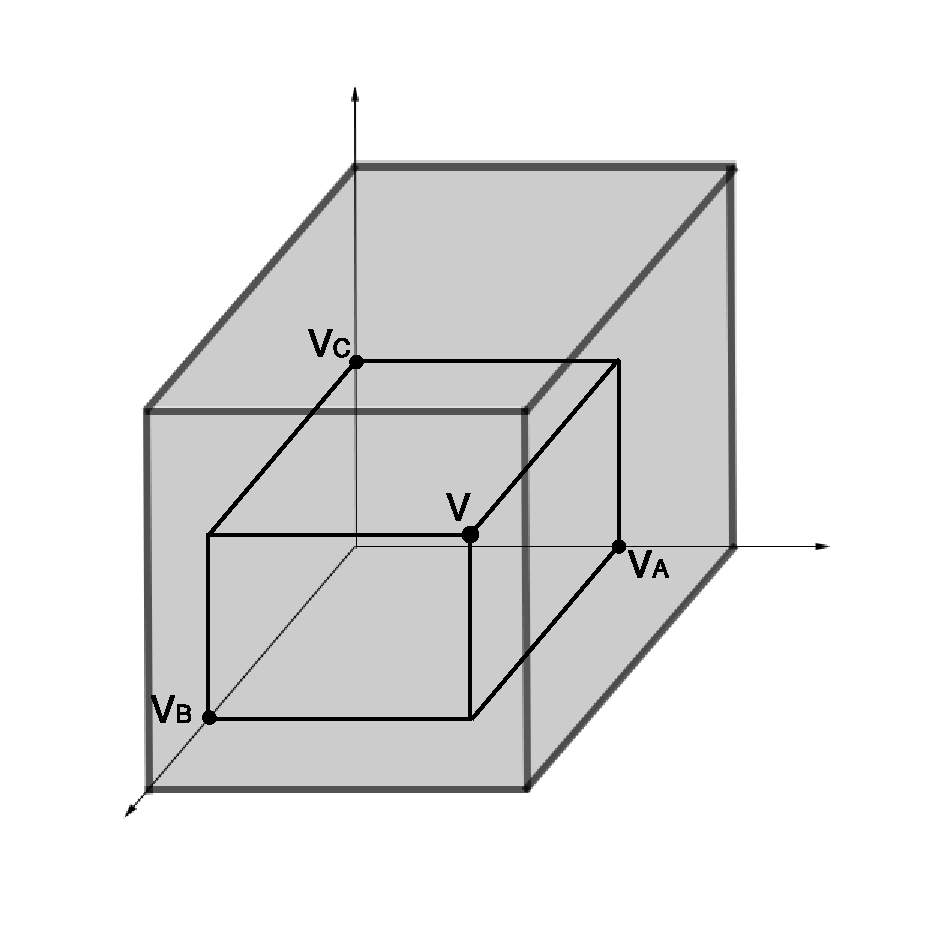
\includegraphics[scale=0.40]{Interpolation-GRID-INS.eps}
\caption{Complete grid, one point case}
\label{figNCRGRIDINS}
\end{center}
\end{figurehere}

\begin{figurehere}
\begin{center}
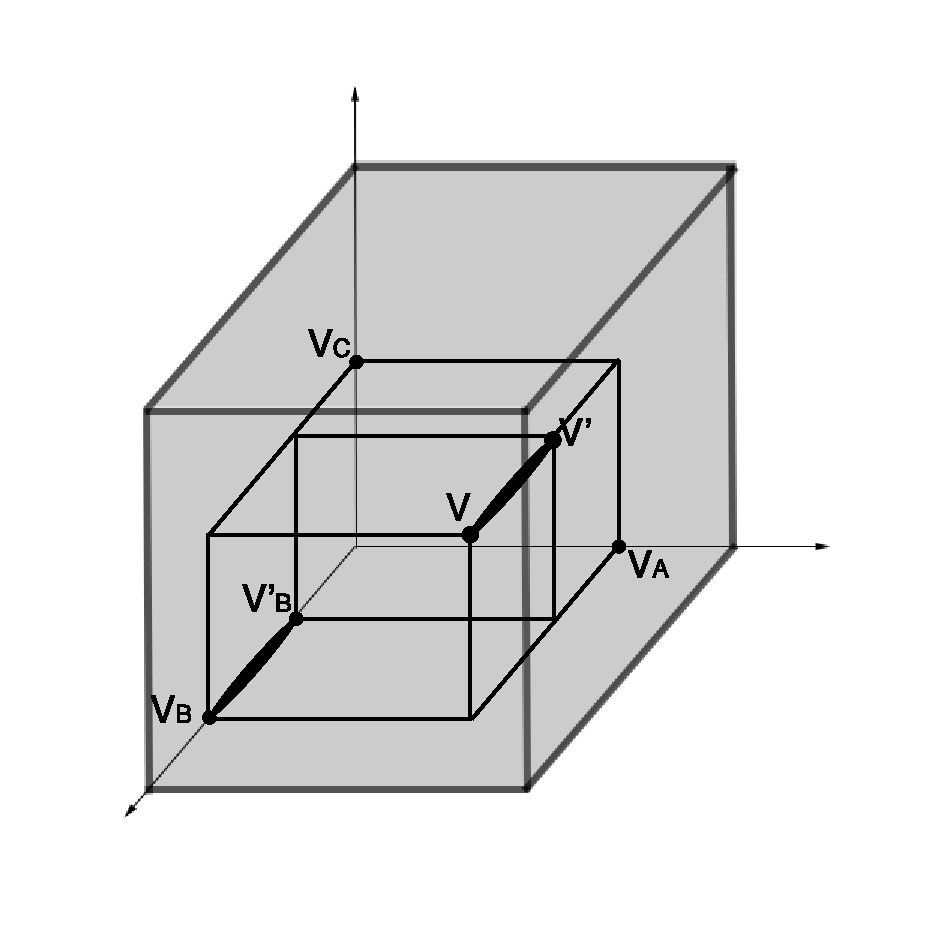
\includegraphics[scale=0.40]{Interpolation-GRID-TA.eps}
\caption{Complete grid, TA case}
\label{figNCRGRIDTA}
\end{center}
\end{figurehere}

\begin{figurehere}
\begin{center}
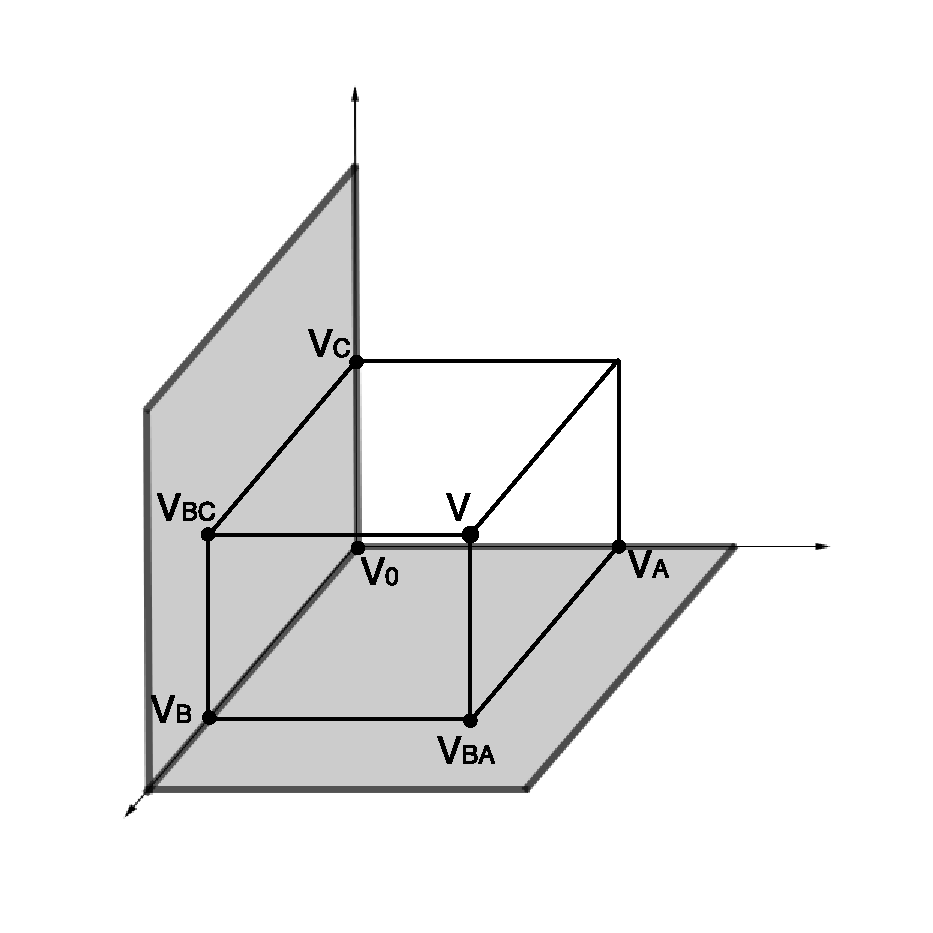
\includegraphics[scale=0.40]{Interpolation-PLANE-INS.eps}
\caption{Partial grid, complete planes, one point case}
\label{figNCRPLANEINS}
\end{center}
\end{figurehere}

\begin{figurehere}
\begin{center}
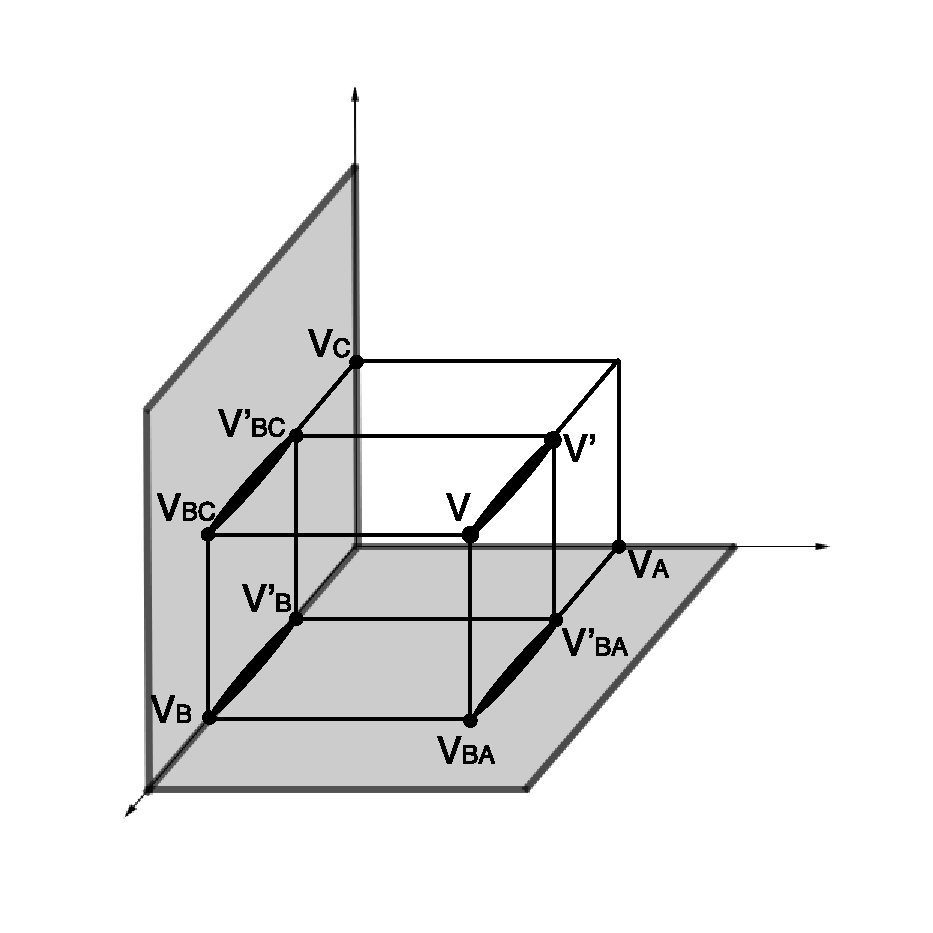
\includegraphics[scale=0.40]{Interpolation-PLANE-TA.eps}
\caption{Partial grid, complete planes, TA case}
\label{figNCRPLANETA}
\end{center}
\end{figurehere}

\begin{figurehere}
\begin{center}
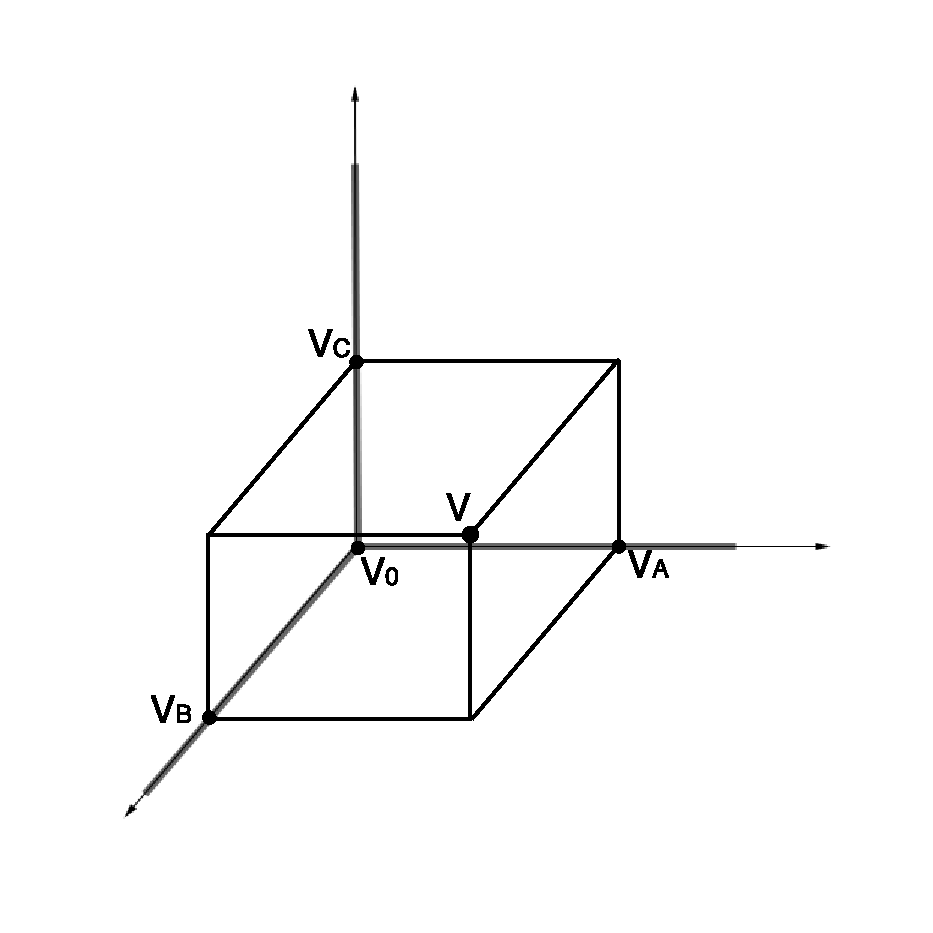
\includegraphics[scale=0.40]{Interpolation-AXE-INS.eps}
\caption{Partial grid, complete axis, one point case}
\label{figNCRAXEINS}
\end{center}
\end{figurehere}

\begin{figurehere}
\begin{center}
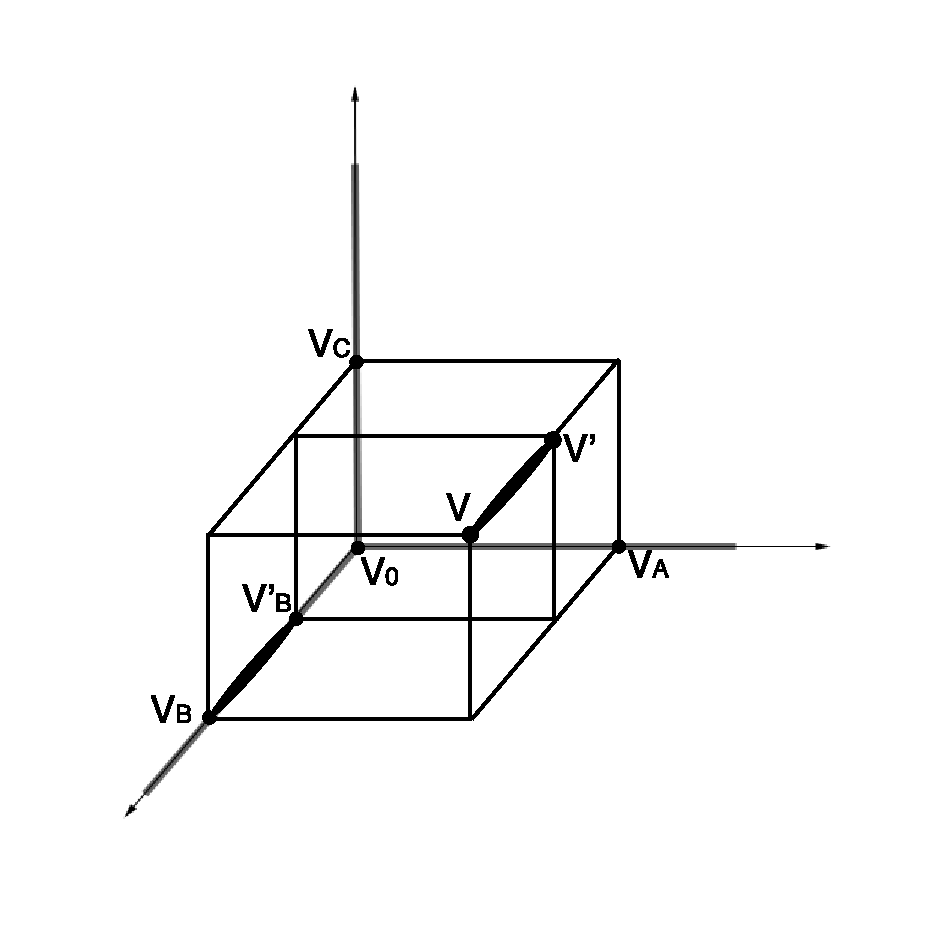
\includegraphics[scale=0.40]{Interpolation-AXE-TA.eps}
\caption{Partial grid, complete axis, TA case}
\label{figNCRAXETA}
\end{center}
\end{figurehere}

\begin{figurehere}
\begin{center}
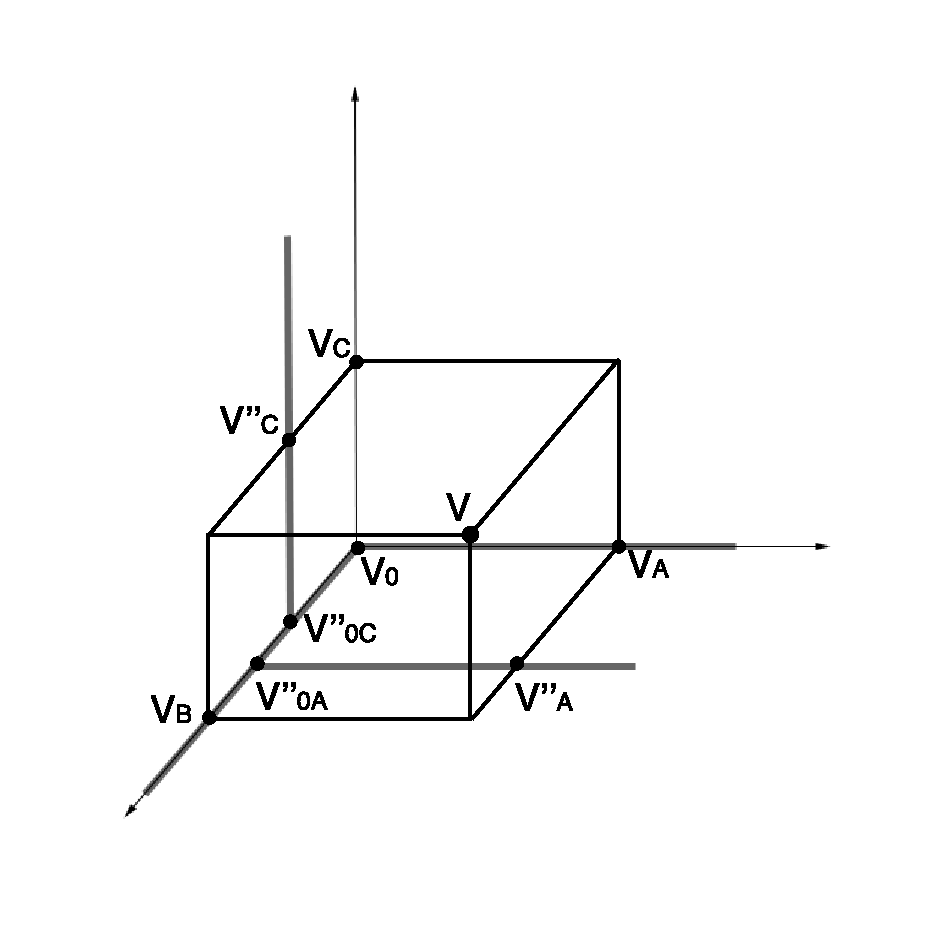
\includegraphics[scale=0.40]{Interpolation-AXE-INSbis.eps}
\caption{Partial grid, complete axis with another configuration, one point case}
\label{figNCRAXEINSbis}
\end{center}
\end{figurehere}

\begin{figurehere}
\begin{center}
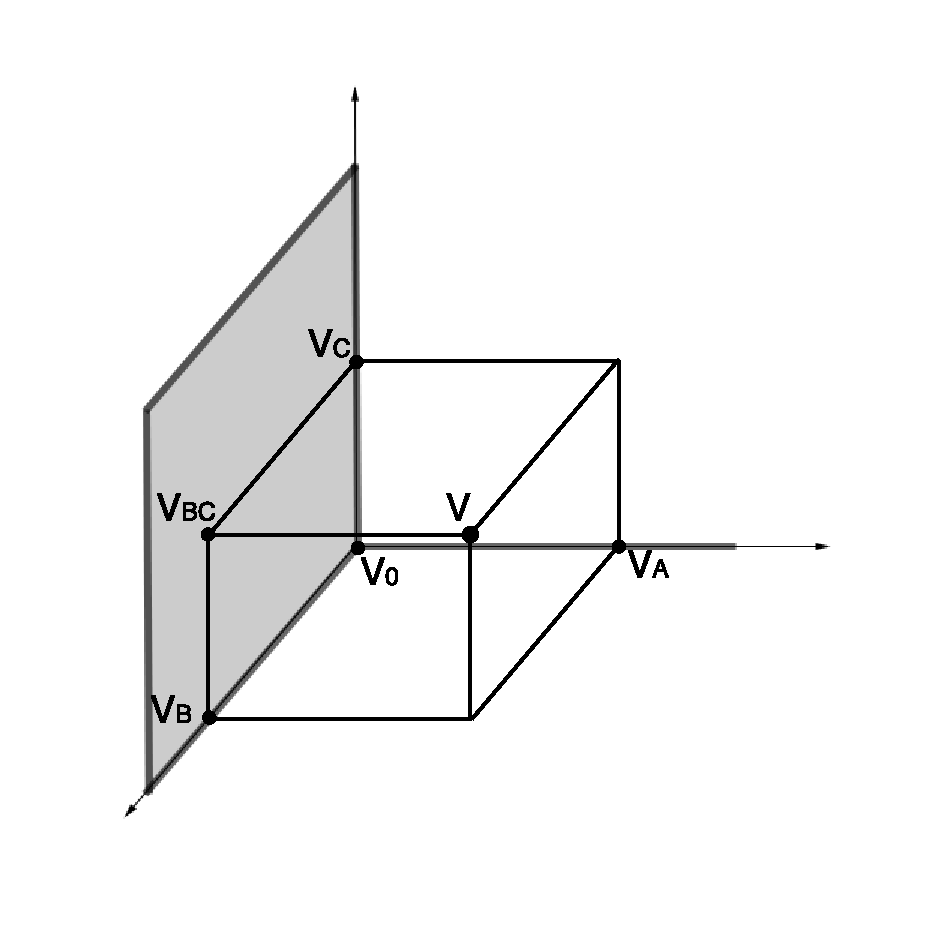
\includegraphics[scale=0.40]{Interpolation-PLAX-INS.eps}
\caption{Partial grid, one complete plane and one complete axis, one point case}
\label{figNCRPLAXINS}
\end{center}
\end{figurehere}

\begin{figurehere}
\begin{center}
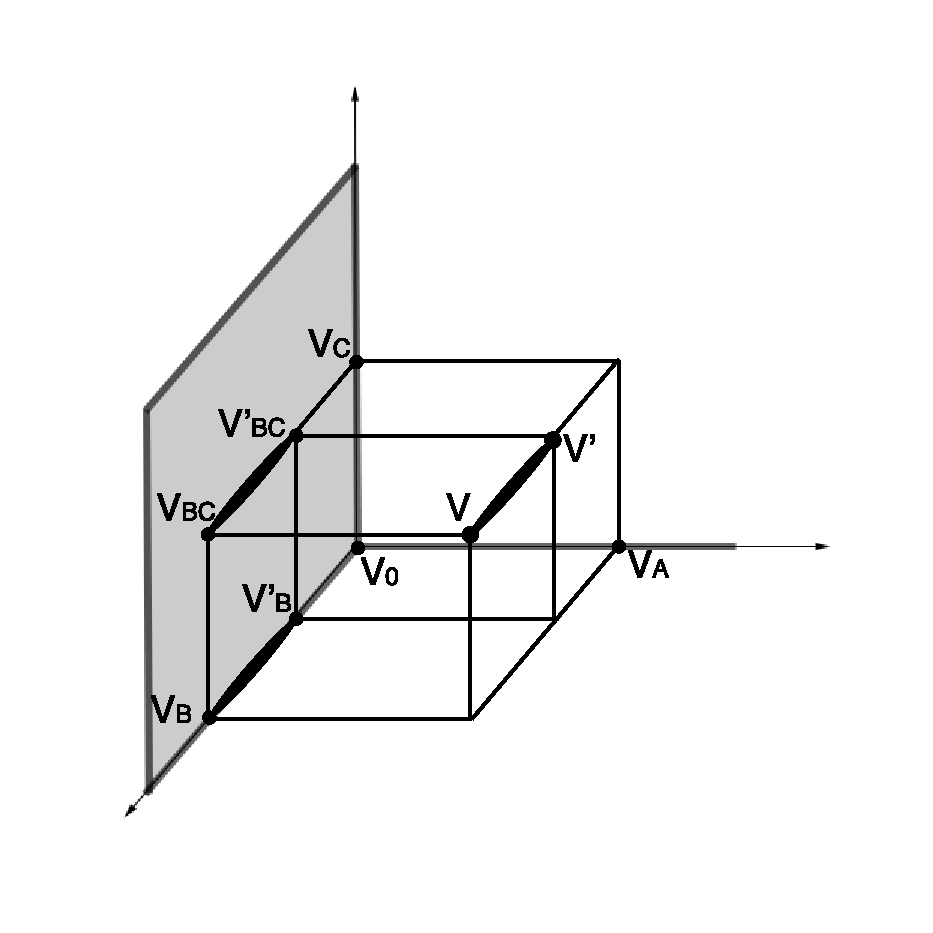
\includegraphics[scale=0.40]{Interpolation-PLAX-TA.eps}
\caption{Partial grid, one complete plane and one complete axis, TA case}
\label{figNCRPLAXTA}
\end{center}
\end{figurehere}

\begin{figurehere}
\begin{center}
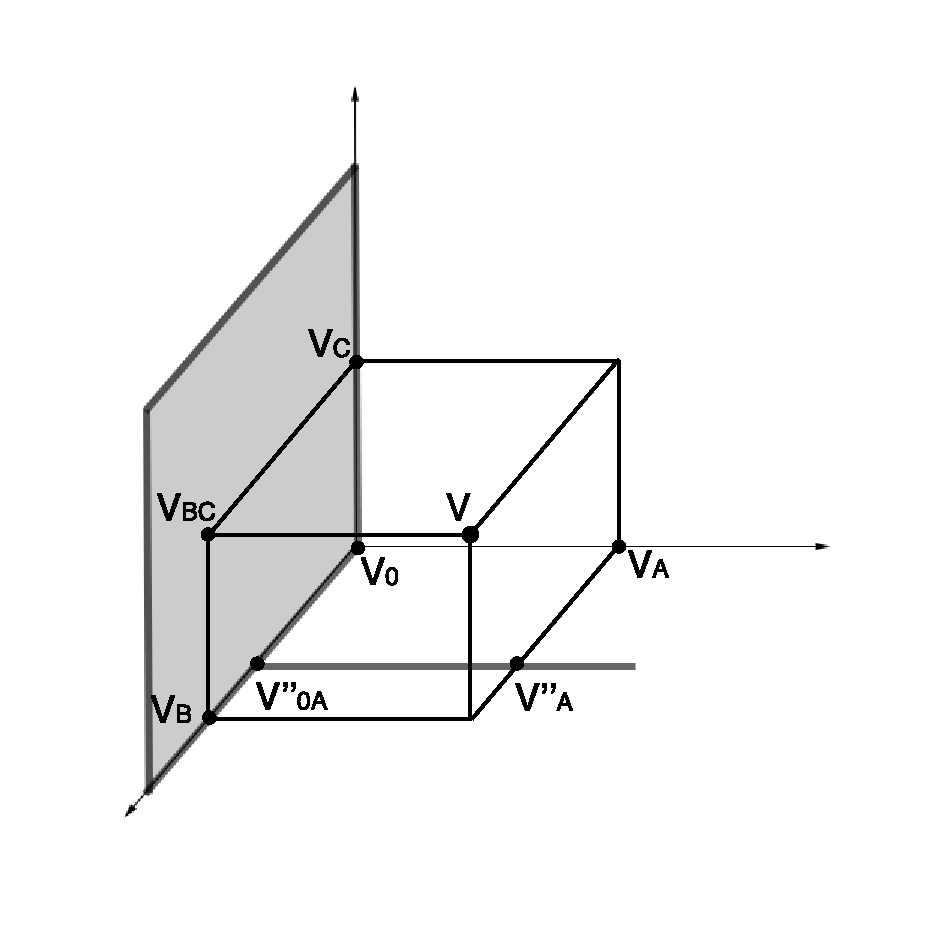
\includegraphics[scale=0.40]{Interpolation-PLAX-INSbis.eps}
\caption{Partial grid, one complete plane and one complete axis with another configuration, one point case}
\label{figNCRPLAXINSbis}
\end{center}
\end{figurehere}

}
\end{multicols}

\clearpage
